\section{Experiments}
\label{sec:experiments}

We study \gls{CVI} with two models: Gaussian mixtures and the latent
space model~\citep{hoff2001latent}. The Gaussian mixture is a
classical example of a model for which it is difficult to capture
posterior dependencies. The latent space model is a modern Bayesian
model for which the mean-field approximation gives poor estimates of
the posterior, and where modeling posterior dependencies is crucial for uncovering patterns in the data.

There are several implementation details of \gls{CVI}. At each
iteration, we form a stochastic gradient by generating $m$ samples
from the variational distribution and taking the average gradient. We
set $m=1024$ and follow asynchronous updates~\citep{recht2011hogwild}. We set the step-size using ADAM~\citep{kingma2015adam}.

\subsection{Mixture of Gaussians}
\label{subsec:mixture}
We follow the goal of \citet{giordano2015linear}, which is to estimate
the posterior covariance for a Gaussian mixture. The hidden variables
are a $K$-vector of mixture proportions $\mbpi$ and a set of $K$
$P$-dimensional multivariate normals
$\mathcal{N}(\mbmu_k,\mbLambda_k^{-1})$, each with unknown mean
$\mbmu_k$ (a $P$-vector) and $P\times P$ precision matrix
$\mbLambda_k$. In a mixture of Gaussians, the joint probability is
\begin{align*}
p(\mbx, \mbz, \mbmu, \mbLambda^{-1},\mbpi)
&= p(\mbpi)\prod_{k=1}^Kp(\mbmu_k,\mbLambda^{-1}_k)\prod_{n=1}^N p(\mbx_n\g
\mbz_n,\mbmu_{\mbz_n},\mbLambda^{-1}_{\mbz_n})p(\mbz_n\g \mbpi),
\end{align*}
with a Dirichlet prior $p(\mbpi)$ and a normal-Wishart prior
$p(\mbmu_k,\mbLambda_k^{-1})$.

We first apply the mean-field approximation (\glsunset{MF}\gls{MF}),
which assigns independent factors to $\mbmu, \mbpi, \mbLambda$, and
$\mbz$. We then perform \gls{CVI} over the copula-augmented
mean-field distribution, i.e., one which includes pair copulas over
the latent variables. We also compare our results to
\gls{LRVB}~\citep{giordano2015linear}, which is a posthoc correction
technique for covariance estimation in variational inference.
Higher-order mean-field methods demonstrate similar behavior as
\gls{LRVB}. Comparisons to structured approximations are omitted as
they require explicit factorizations and are not black box. Standard black box variational inference~\citep{ranganath2014black}
corresponds to the \gls{MF} approximation.

\begin{figure}[t]
  \centering
  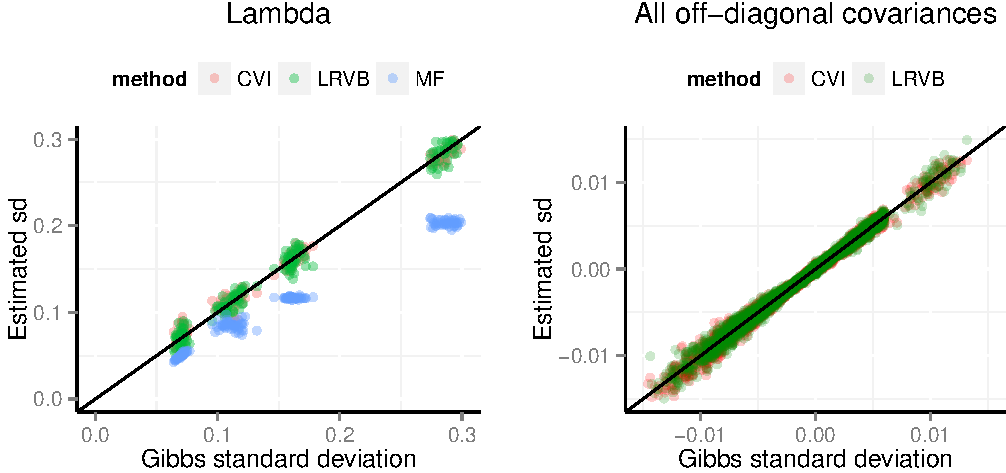
\includegraphics[width=0.7\textwidth]{img/mixture_gaussians.pdf}
  \caption{\label{fig:lrvb}Covariance estimates from
  copula variational inference (\gls{CVI}), mean-field (\gls{MF}), and
  linear response variational Bayes (\gls{LRVB}) to the ground truth
  (Gibbs samples). \gls{CVI} and \gls{LRVB} effectively capture dependence
  while \gls{MF} underestimates variance and forgets covariances.}
\end{figure}

We simulate $10,000$ samples with $K=2$ components and $P=2$
dimensional Gaussians. Figure \ref{fig:lrvb} displays estimates for
the standard deviations of $\mbLambda$ for 100 simulations, and plots
them against the ground truth using 500 effective Gibb samples. The
second plot displays all off-diagonal covariance estimates. Estimates
for $\mbmu$ and $\mbpi$ indicate the same pattern and are given in the
supplement.

When initializing at the true mean-field parameters, both \gls{CVI}
and \gls{LRVB} achieve consistent estimates of the posterior variance. \gls{MF} underestimates the variance, which is a well-known
limitation~\citep{wainwright2008graphical}. Note that
because the \gls{MF} estimates are initialized at the truth, \gls{CVI}
converges to the true posterior upon one step of fitting the copula. It does not require alternating more steps.

\Gls{CVI} is more robust than \gls{LRVB}. As a toy demonstration, we
analyze the MNIST data set of handwritten digits, using 12,665
training examples and 2,115 test examples of 0's and 1's. We perform
"unsupervised" classification, i.e., classify without using training
labels: we apply a mixture of Gaussians to cluster, and then classify
a digit based on its membership assignment. \gls{CVI} reports a test
set error rate of 0.06, whereas \gls{LRVB} ranges between 0.06 and
0.32 depending on the mean-field estimates. \gls{LRVB} and similar
higher order mean-field methods correct an existing \gls{MF}
solution---it is thus sensitive to local optima and the general
quality of that solution. On the other hand, \gls{CVI} re-adjusts both
the \gls{MF} and copula parameters as it fits, making it more robust
to initialization.

\subsection{Latent space model}
\label{subsec:latent}

We next study inference on the latent space
model~\citep{hoff2001latent}, a Bernoulli latent factor model for
network analysis. Each node in an $N$-node network is associated with
a $P$-dimensional latent variable $\mbz\sim N(\mbmu,\mbLambda^{-1})$.
Edges between pairs of nodes are observed with high probability if the
nodes are close to each other in the latent space. Formally, an edge
for each pair $(i,j)$ is observed with probability $\mathrm{logit}(p)=
\theta - |\mbz_i - \mbz_j|$, where $\theta$ is a model parameter.

We generate an $N=100,000$ node network with latent node attributes
from a $P=10$ dimensional Gaussian. We learn the posterior of the
latent attributes in order to predict the likelihood of held-out
edges. \gls{MF} applies independent factors on $\mbmu,
\mbLambda,\theta$ and $\mbz$, \gls{LRVB} applies a correction, and
\gls{CVI} uses the fully dependent variational distribution. Table
\ref{table:latent} displays the likelihood of held-out edges and runtime. We also attempted Hamiltonian Monte Carlo but it did not
converge after five hours.

\Gls{CVI} dominates other methods in accuracy upon convergence, and
the copula estimation without refitting (2 steps) already dominates
\gls{LRVB} in both runtime and accuracy. We note however that
\gls{LRVB} requires one to invert a
$\mathcal{O}(NK^3)\times\mathcal{O}(NK^3)$ matrix. We can better scale
the method and achieve faster estimates than \gls{CVI} if we applied
stochastic approximations for the inversion. However, \gls{CVI} always
outperforms \gls{LRVB} and is still fast on this 100,000 node network.

\begin{table}[t]
  \centering
  \begin{tabular}{lll}
  \toprule
  Variational inference methods & Predictive Likelihood & Runtime\\
  \midrule
  {Mean-field} & -383.2 & 15 min.\\
  \gls{LRVB} & -330.5 & 38 min.\\
  \gls{CVI} (2 steps) & -303.2 & 32 min.\\
  \gls{CVI} (5 steps) & -80.2 & 1 hr. 17 min.\\
  \gls{CVI} (converged) & -50.5 & 2 hr.\\
  \bottomrule
  \end{tabular}
  \captionof{table}{\label{table:latent}Predictive likelihood on the
  latent space model. Each \gls{CVI} step either refits the mean-field
  or the copula. \gls{CVI} converges in roughly 10 steps and already
  significantly outperforms both mean-field and \gls{LRVB} upon
  fitting the copula once (2 steps).}
\end{table}


%%% Local Variables:
%%% mode: latex
%%% TeX-master: "nips2015"
%%% End:
